\begin{figure}
    \begin{tikzpicture}[scale=1.5]
        \def\mriwidth{8cm}
        \node[inner sep=0pt, outer sep=0pt] (zeroth) at (0, 0) {
            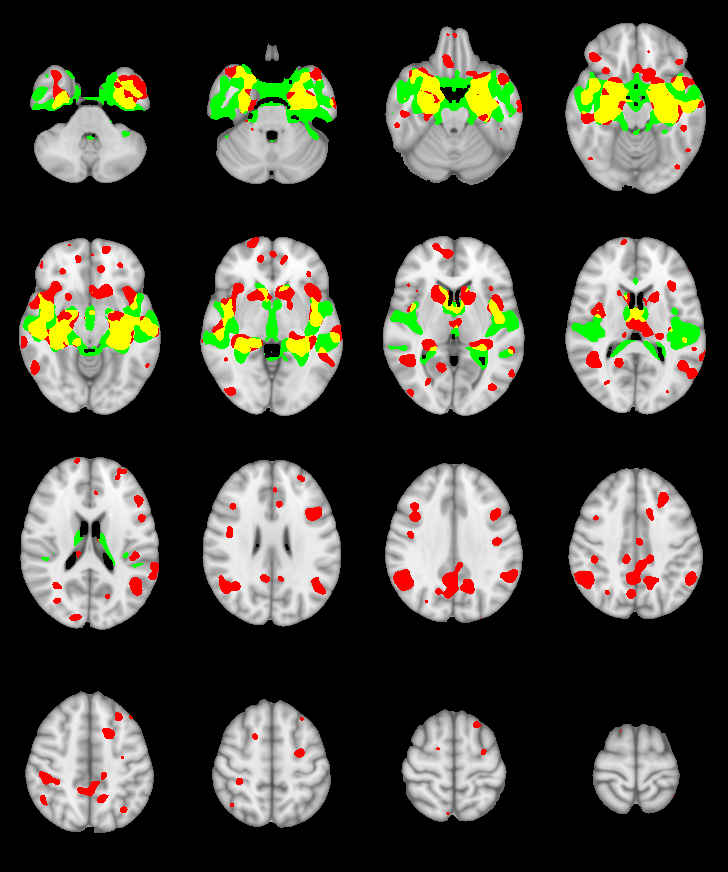
\includegraphics[
                height=\mriwidth,
                clip=true,
                trim = 128mm 237mm 64mm 5mm
            ]{data/test_90.png}
        };
        \node[inner sep=0pt, outer sep=0pt, anchor=west] (first) at (zeroth.east) {
            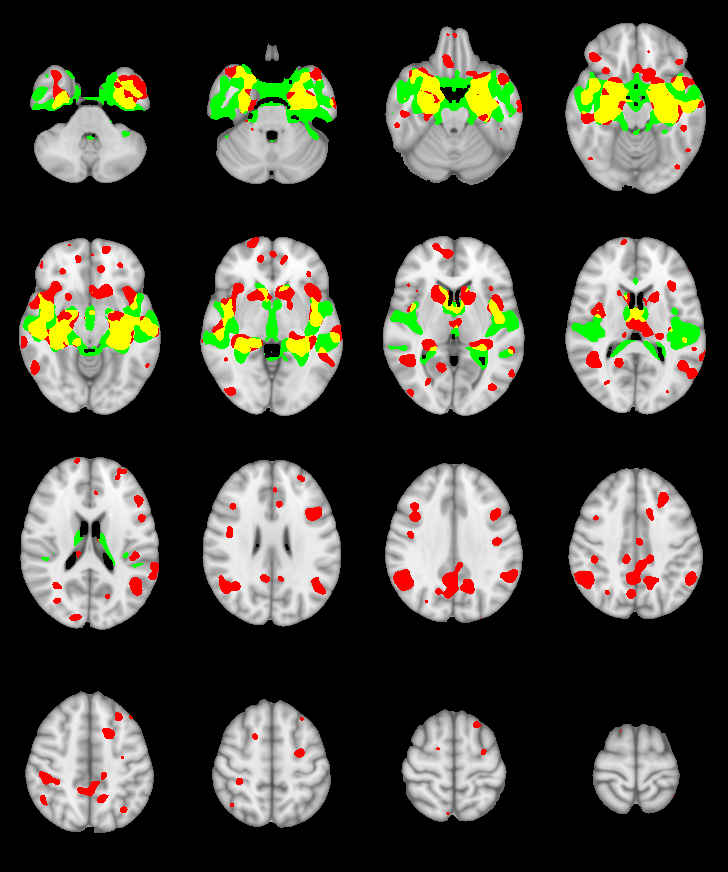
\includegraphics[
                height=\mriwidth,
                clip=true,
                trim = 192mm 237mm 0mm 5mm
            ]{data/test_90.png}
        };
        \node[inner sep=0pt, outer sep=0pt, anchor=west] (second) at (first.east) {
            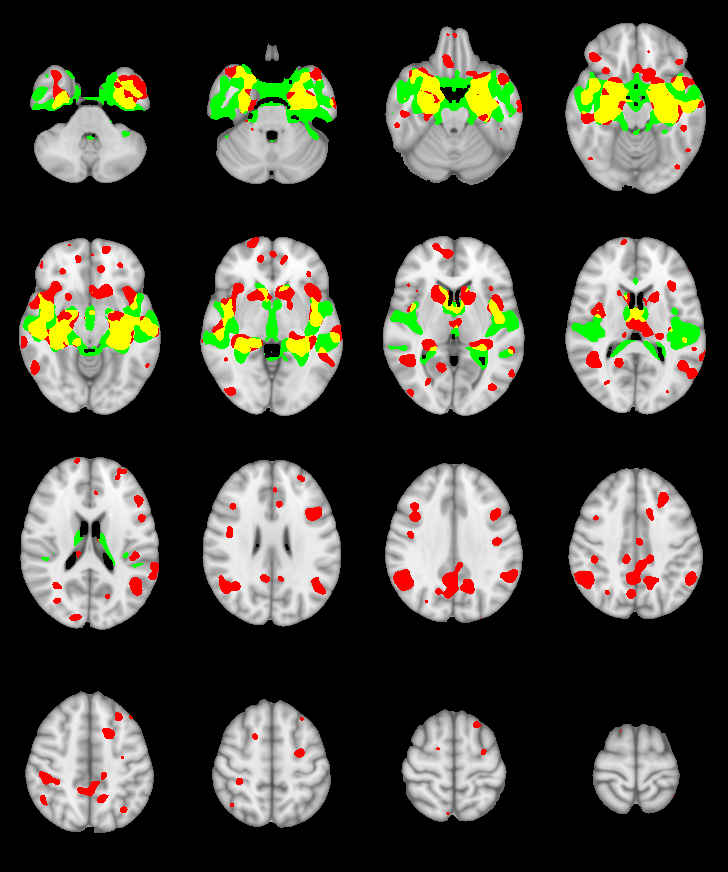
\includegraphics[
                height=\mriwidth,
                clip=true,
                trim = 0mm 162mm 192mm 82mm
            ]{data/test_90.png}
        };
        \draw[fill=black] (zeroth.north west) -- (second.north east) -- ($ (second.south east) - (0, 1) $) -- ($ (zeroth.south west) -(0, 1) $) -- cycle;
        \node[inner sep=0pt, outer sep=0pt] (zeroth) at (0, 0) {
            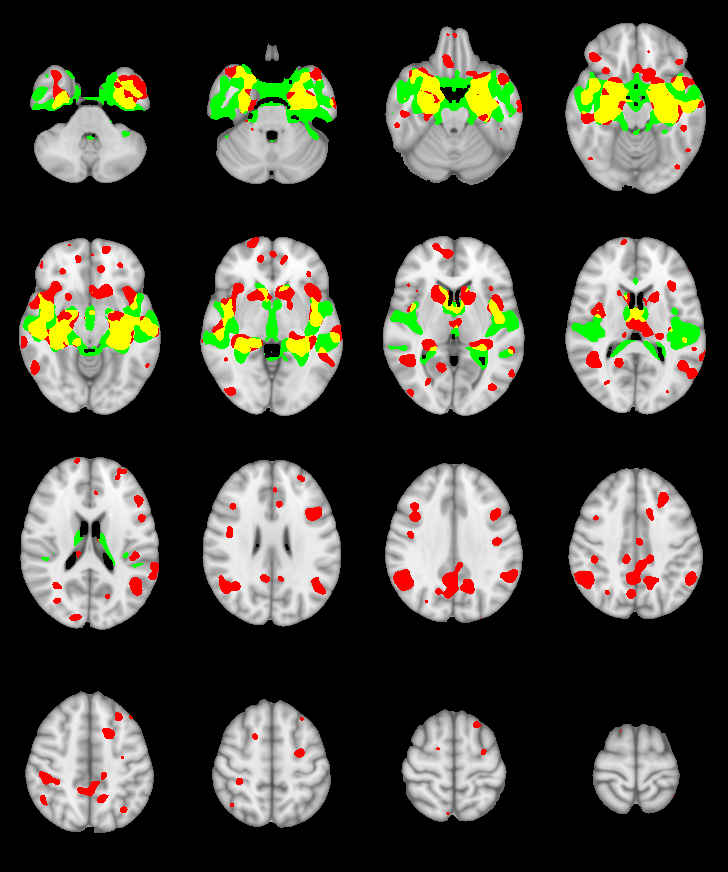
\includegraphics[
                height=\mriwidth,
                clip=true,
                trim = 128mm 237mm 64mm 5mm
            ]{data/test_90.png}
        };
        \node[inner sep=0pt, outer sep=0pt, anchor=west] (first) at (zeroth.east) {
            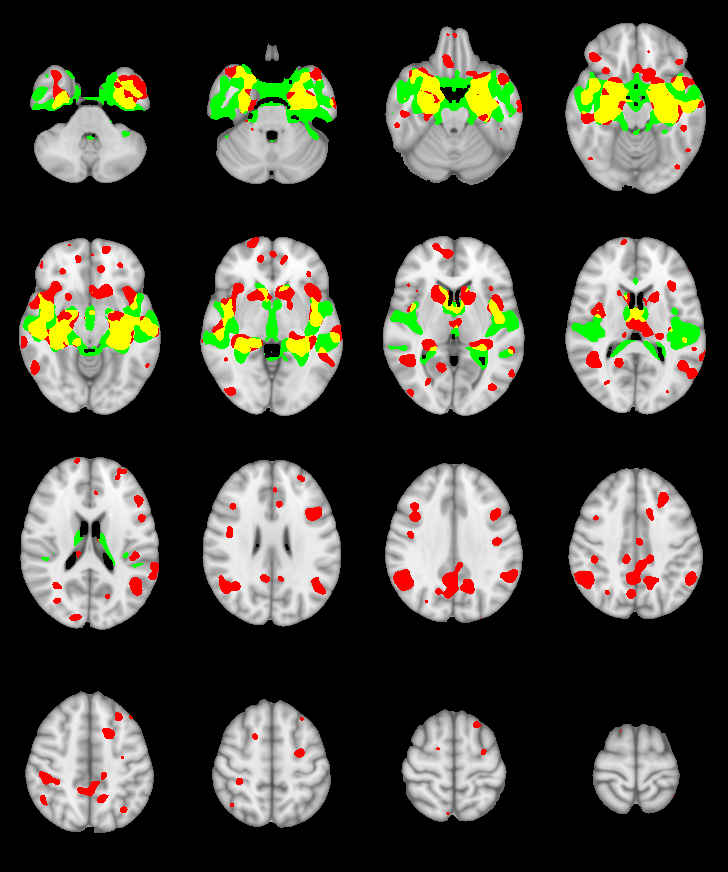
\includegraphics[
                height=\mriwidth,
                clip=true,
                trim = 192mm 237mm 0mm 5mm
            ]{data/test_90.png}
        };
        \node[inner sep=0pt, outer sep=0pt, anchor=west] (second) at (first.east) {
            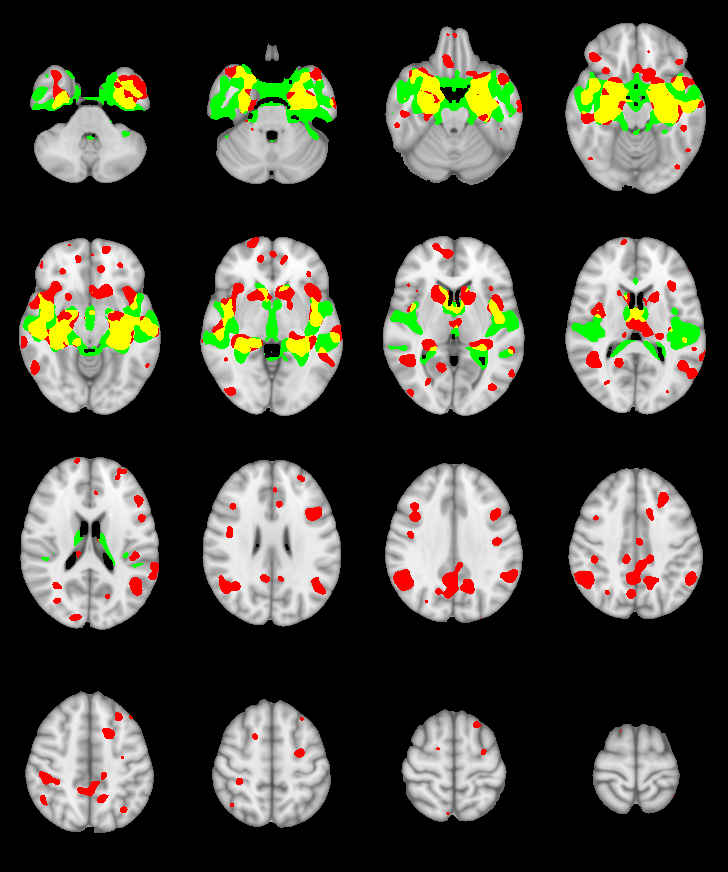
\includegraphics[
                height=\mriwidth,
                clip=true,
                trim = 0mm 162mm 192mm 82mm
            ]{data/test_90.png}
        };

        \node[text=white, text depth=0] at ($ (first.south) - (0, 0.5) $) (overlap-text) {Overlap};
        \node[fill=yellow, anchor=east] at ($ (overlap-text.west) - (0.2, 0) $) (overlap) {};
        \node[text=white, text depth=0, anchor=east] at ($ (overlap.west) - (0.4, 0) $) (lrp-text) {LRP};
        \node[fill=green, anchor=east] at ($ (lrp-text.west) - (0.2, 0) $) (lrp) {};
        \node[fill=red, anchor=west] at ($ (overlap-text.east) + (0.4, 0) $) (ale) {};
        \node[text=white, text depth=0, anchor=west] at ($ (ale.east) + (0.2, 0) $) (ale-text) {ALE};
        \node[font=\fontsize{24}{28}\selectfont\itshape, anchor=north] at ($ (first.south) - (0, 1.1) $) {
            \textbf{Figure 2: Overlap between the average and reference heatmaps.}
        };
    \end{tikzpicture}
\end{figure}
